\documentclass[aspectratio=169,11pt]{beamer}
\usepackage[T1]{fontenc}
\usepackage{lmodern}
\usepackage{amsmath,amssymb,booktabs,listings}
\usetheme{Madrid}
\usecolortheme{dolphin}
\setbeamertemplate{blocks}[rounded][shadow=false]
\definecolor{Navy}{HTML}{15345C}
\definecolor{Teal}{HTML}{2266B3}
\definecolor{Coral}{HTML}{D6603C}
\definecolor{Mist}{HTML}{EFF5FC}
\setbeamercolor{normal text}{fg=Navy,bg=white}
\setbeamercolor{structure}{fg=Teal}
\setbeamercolor{frametitle}{fg=white,bg=Navy}
\setbeamercolor{title}{fg=white,bg=Navy}
\setbeamercolor{subtitle}{fg=white}
\setbeamercolor{alerted text}{fg=Teal}
\setbeamercolor{palette primary}{fg=white,bg=Teal}
\setbeamercolor{palette secondary}{fg=white,bg=Navy}
\setbeamercolor{palette tertiary}{fg=white,bg=Navy}
\setbeamercolor{block title}{fg=white,bg=Teal}
\setbeamercolor{block body}{fg=Navy,bg=Mist}
\setbeamerfont{title}{size=\Huge,series=\bfseries}
\setbeamerfont{frametitle}{size=\Large,series=\bfseries}
\setbeamertemplate{navigation symbols}{}
\setbeamertemplate{itemize items}[circle]
\setbeamersize{text margin left=9mm,text margin right=9mm}
\setbeamertemplate{headline}{}
\setbeamertemplate{footline}{%
 \leavevmode\hbox{%
 \begin{beamercolorbox}[wd=.84\paperwidth,ht=2.8ex,dp=1.2ex,leftskip=9mm]{palette secondary}%
 \scriptsize DRP\enspace\textbar\enspace Diffusion and Flow Matching
 \end{beamercolorbox}%
 \begin{beamercolorbox}[wd=.16\paperwidth,ht=2.8ex,dp=1.2ex,center]{palette primary}%
 \scriptsize\insertframenumber\,/\,\inserttotalframenumber
 \end{beamercolorbox}}}
\lstset{language=Python,basicstyle=\ttfamily\small,keywordstyle=\color{Teal}\bfseries,
 stringstyle=\color{Coral},showstringspaces=false,columns=fullflexible,keepspaces=true,
 frame=none,backgroundcolor=\color{Mist},xleftmargin=2mm,xrightmargin=2mm,
 aboveskip=3mm,belowskip=3mm,breaklines=false}
\newcommand{\fmref}{\vfill{\tiny\color{gray}Lipman et al., \href{https://arxiv.org/abs/2210.02747}{Flow Matching for Generative Modeling}; Liu et al., \href{https://arxiv.org/abs/2209.03003}{Rectified Flow}.}}
\title{Diffusion models\\and ODE generation}
\subtitle{A simple flow-matching example with four Gaussian components}
\author{\texorpdfstring{Directed Reading Program\\Florida State University}{Directed Reading Program, Florida State University}}
\date{}
\begin{document}

\begin{frame}
\titlepage
\vspace{-5mm}
\centering\textcolor{Teal}{Data \quad Velocity \quad Training \quad ODE sampling}
\end{frame}

\begin{frame}{Our goal: generate a mixture from Gaussian noise}
\large
\[X(0)\sim\mathcal N(0,I_2)\]
\[X(1)\ \text{approximately follows}\quad
\frac14\sum_{j=1}^4\mathcal N(\mu_j,0.35^2I_2)\]
\normalsize
\begin{itemize}\setlength\itemsep{4mm}
\item One sample is a point with two coordinates.
\item We learn a velocity field that moves a cloud of points.
\item A fresh Gaussian starting point produces a new generated sample.
\end{itemize}
\end{frame}

\begin{frame}{What is a four-component Gaussian mixture?}
\[\mu_1=(-2,-2),\quad\mu_2=(-2,2),\quad
\mu_3=(2,-2),\quad\mu_4=(2,2)\]
\vspace{3mm}
\begin{enumerate}\setlength\itemsep{4mm}
\item Choose one center with probability $1/4$.
\item Draw $\varepsilon\sim\mathcal N(0,I_2)$.
\item Return $x=\mu_j+0.35\varepsilon$.
\end{enumerate}
\vspace{5mm}
The covariance is $0.35^2 I_2$. Each cluster has width, not just a single point.\\[3mm]
Direct sampling already works. We use the known mixture to teach and check a learned generator.
\end{frame}

\begin{frame}[fragile]{1. Create the training data}
\begin{columns}[c]
\begin{column}{.55\textwidth}
\begin{lstlisting}[basicstyle=\ttfamily\footnotesize]
centers = torch.tensor([
    [-2., -2.], [-2., 2.],
    [2., -2.], [2., 2.]
])
sigma = 0.35

def sample_data(n):
    labels = torch.randint(4, (n,))
    return (centers[labels]
            + sigma * torch.randn(n, 2))

x_train = sample_data(4096)
\end{lstlisting}
\small Shape: \texttt{(4096, 2)}. The network receives samples, not their component labels.
\end{column}
\begin{column}{.42\textwidth}
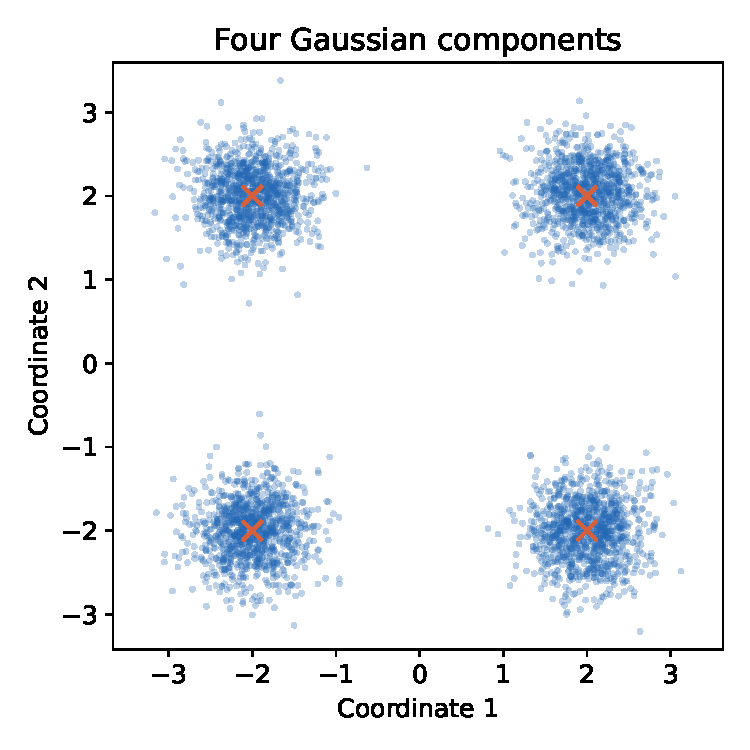
\includegraphics[width=\linewidth]{figures/training_data.pdf}
\end{column}
\end{columns}
\end{frame}

\begin{frame}{An ODE specifies how a point moves}
\large
\[\boxed{\frac{dX(t)}{dt}=v_\theta(X(t),t)}\]
\normalsize
\begin{itemize}\setlength\itemsep{4mm}
\item $X(t)$ is the current position in the plane.
\item $v_\theta(x,t)$ is a two-dimensional velocity.
\item $\theta$ contains the network's weights and biases.
\end{itemize}
\vspace{4mm}
Our convention: $t=0$ means noise and $t=1$ means data.\\[3mm]
This is \alert{generation time}, not physical time or a time-series index.
\end{frame}

\begin{frame}{One Euler step}
\large
\[X_{k+1}=X_k+\Delta t\,v_\theta(X_k,t_k)\]
\normalsize
\vspace{3mm}
An illustrative calculation:
\[X_k=(0,1),\qquad v_\theta(X_k,t_k)=(2,-1),\qquad\Delta t=0.1\]
\[X_{k+1}=(0,1)+0.1(2,-1)=(0.2,0.9).\]
\vspace{4mm}
We approximate a short motion using the velocity at the start of the step.\\[3mm]
At the next step, evaluate the velocity at the new position and time.
\end{frame}

\begin{frame}{Diffusion and flow matching: related approaches}
\begin{center}
\small
\begin{tabular}{p{.22\textwidth}p{.32\textwidth}p{.32\textwidth}}
\toprule
& Score-based diffusion & This notebook\\\midrule
Training construction & Add noise to data & Interpolate noise and data\\[3mm]
Learned quantity & Score $\nabla_x\log p_t(x)$ & Velocity $v_\theta(x,t)$\\[3mm]
Generation & Reverse SDE or probability-flow ODE & Forward ODE from noise to data\\\bottomrule
\end{tabular}
\end{center}
\vspace{4mm}
We implement \alert{flow matching}, not a DDPM or Brownian-motion simulation.\\[3mm]
The ODE makes the transport idea accessible with basic calculus.
\fmref
\end{frame}

\begin{frame}{2. Construct straight training paths}
Choose independently:
\[x_0\sim\mathcal N(0,I_2),\qquad x_1\sim\text{training data},\qquad t\sim U[0,1].\]
\large
\[\boxed{x_t=(1-t)x_0+tx_1}\]
\normalsize
\begin{center}
\begin{tabular}{ccc}
\toprule
$t=0$ & $t=1/2$ & $t=1$\\\midrule
$x_0$ & $(x_0+x_1)/2$ & $x_1$\\\bottomrule
\end{tabular}
\end{center}
\vspace{5mm}
We can sample a point on this path directly, without solving an ODE.
\fmref
\end{frame}

\begin{frame}{The target velocity is easy to calculate}
\large
\[\frac{d}{dt}\bigl((1-t)x_0+tx_1\bigr)=x_1-x_0\]
\[\boxed{u=x_1-x_0}\]
\normalsize
\vspace{3mm}
Example: $x_0=(0,0)$ and $x_1=(2,2)$.\\[3mm]
At $t=0.25$, the position is $x_t=(0.5,0.5)$ and the target velocity is $(2,2)$.\\[4mm]
The position changes along this training segment. Its target velocity stays constant.
\end{frame}

\begin{frame}{What does the network learn from many pairs?}
Different noise-data pairs can give the same $(x_t,t)$ with different velocities.
\vspace{4mm}
\large
\[v^*(x,t)=\mathbb E[X_1-X_0\mid X_t=x]\]
\normalsize
\vspace{4mm}
Squared-error regression learns the conditional average velocity.\\[3mm]
Under suitable regularity assumptions, the ideal field transports the interpolation distributions.\\[3mm]
The learned ODE paths need not be straight or end at a paired training sample.
\fmref
\end{frame}

\begin{frame}[fragile]{3. A network for position and time}
\begin{columns}[c]
\begin{column}{.48\textwidth}
\begin{lstlisting}
model = nn.Sequential(
    nn.Linear(3, 64),
    nn.SiLU(),
    nn.Linear(64, 64),
    nn.SiLU(),
    nn.Linear(64, 2)
)
\end{lstlisting}
\end{column}
\begin{column}{.47\textwidth}
\[\text{Input: }(x^{(1)},x^{(2)},t)\]
\[\text{Output: }(v^{(1)},v^{(2)})\]
\small
Two hidden layers of width 64.\\[3mm]
4,546 trainable parameters.\\[3mm]
Smooth activation: $\operatorname{SiLU}(a)=a\sigma(a)$.
\end{column}
\end{columns}
\end{frame}

\begin{frame}[fragile]{Each training row has its own time}
\begin{lstlisting}
t = torch.rand(256, 1)
xt = (1 - t) * x0 + t * x1
prediction = model(torch.cat([xt, t], dim=1))
\end{lstlisting}
\begin{center}
\begin{tabular}{ll}
\toprule
Tensor & Shape\\\midrule
\texttt{x0}, \texttt{x1}, \texttt{xt} & $256\times2$\\[2mm]
\texttt{t} & $256\times1$\\[2mm]
Network input & $256\times3$\\[2mm]
Predicted velocity & $256\times2$\\\bottomrule
\end{tabular}
\end{center}
\small The same location can require different motion at different generation times.
\end{frame}

\begin{frame}[fragile]{4. Mean squared velocity error}
\large
\[L(\theta)=\frac{1}{2B}\sum_{i=1}^B
\left\|v_\theta(x_{t_i},t_i)-(x_{1,i}-x_{0,i})\right\|^2\]
\normalsize
\begin{lstlisting}
loss_fn = nn.MSELoss()
\end{lstlisting}
\vspace{3mm}
PyTorch averages over all $B$ examples and both output coordinates.\\[3mm]
We compare velocities, not generated endpoints.\\[3mm]
The target is a vector with two entries, not a real/fake label.
\end{frame}

\begin{frame}[fragile]{One optimizer updates the velocity network}
\begin{lstlisting}
optimizer = torch.optim.Adam(
    model.parameters(), lr=0.001
)
\end{lstlisting}
\begin{itemize}\setlength\itemsep{4mm}
\item The optimizer adjusts the same weights and biases across all times.
\item Adam uses running averages of gradients and squared gradients.
\item We use its default averaging settings and learning rate 0.001.
\end{itemize}
\vspace{4mm}
There is one regression objective and no discriminator.
\end{frame}

\begin{frame}[fragile]{5. Training: create a batch and predict velocity}
\begin{lstlisting}[basicstyle=\ttfamily\footnotesize]
history = []
for step in range(5000):
    x1 = x_train[torch.randint(len(x_train), (256,))]
    x0 = torch.randn(256, 2)
    t = torch.rand(256, 1)
    xt = (1 - t) * x0 + t * x1
    target = x1 - x0
    prediction = model(torch.cat([xt, t], dim=1))
    loss = loss_fn(prediction, target)
\end{lstlisting}
\vspace{4mm}
Fresh noise and times at each iteration. Real examples sample the training set with replacement.\\[3mm]
The network sees only \texttt{xt} and \texttt{t}.
\end{frame}

\begin{frame}[fragile]{Training: update the parameters}
Continuation inside the same loop:
\begin{lstlisting}
    optimizer.zero_grad()
    loss.backward()
    optimizer.step()
    history.append(loss.item())
\end{lstlisting}
\begin{tabular}{ll}
\texttt{zero\_grad()} & Clear previous gradients.\\[3mm]
\texttt{backward()} & Differentiate the velocity loss.\\[3mm]
\texttt{step()} & Update the network parameters.\\
\end{tabular}

\vspace{5mm}
Training does not require an ODE solve. Sampling will.
\end{frame}

\begin{frame}{Why the loss does not approach zero}
\begin{center}
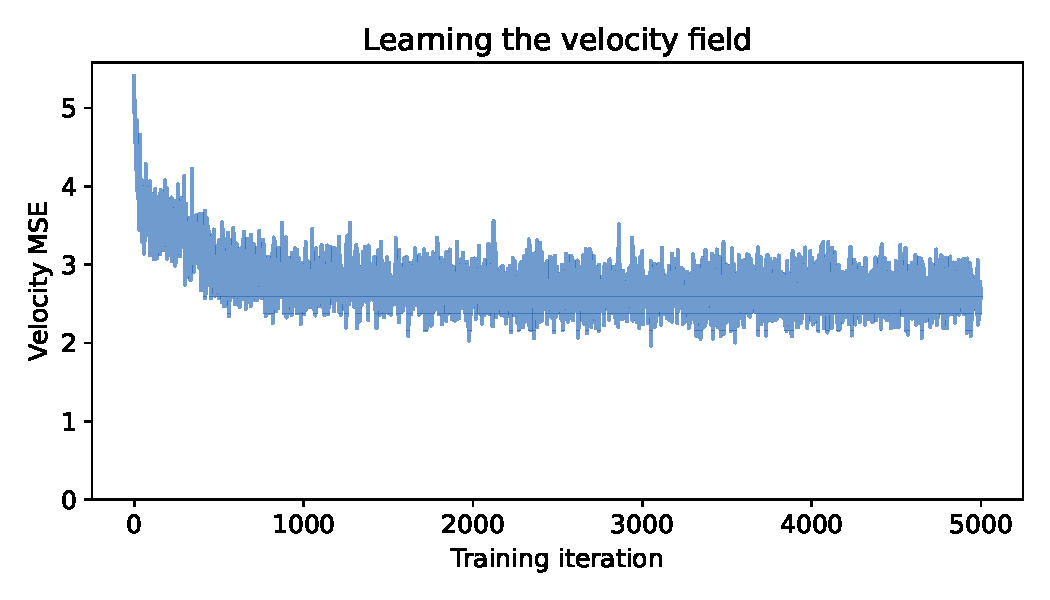
\includegraphics[width=.78\textwidth,height=.61\textheight,keepaspectratio]{figures/loss_curve.pdf}
\end{center}
\small
The target velocity varies across pairs, even at the same position and time.\\[2mm]
The best predictor averages these targets. Their conditional variance leaves residual error.
\end{frame}

\begin{frame}[fragile]{6. ODE sampling with forward Euler}
\begin{lstlisting}[basicstyle=\ttfamily\footnotesize]
def generate(z, steps=100):
    x = z.clone()
    path = [x.clone()]
    with torch.no_grad():
        for k in range(steps):
            t = torch.full((len(x), 1), k / steps)
            x = x + model(torch.cat([x, t], dim=1)) / steps
            path.append(x.clone())
    return x, torch.stack(path)
\end{lstlisting}
\vspace{3mm}
$\Delta t=1/\texttt{steps}$. The plus sign advances from noise to data.\\[2mm]
The model stays fixed. We record positions only to visualize the trajectories.
\end{frame}

\begin{frame}[fragile]{A fresh Gaussian input gives a new sample}
\begin{lstlisting}
torch.manual_seed(2026)
model.eval()
z = torch.randn(5000, 2)
real_test = sample_data(5000)
generated, path = generate(z)
\end{lstlisting}
\vspace{3mm}
The sampler uses Gaussian inputs, time, and the learned velocity network.\\[3mm]
\texttt{real\_test} is only for evaluation; it never enters \texttt{generate}.\\[3mm]
The same input and fixed model give the same numerical trajectory.
\end{frame}

\begin{frame}{The cloud evolves into four clusters}
\begin{center}
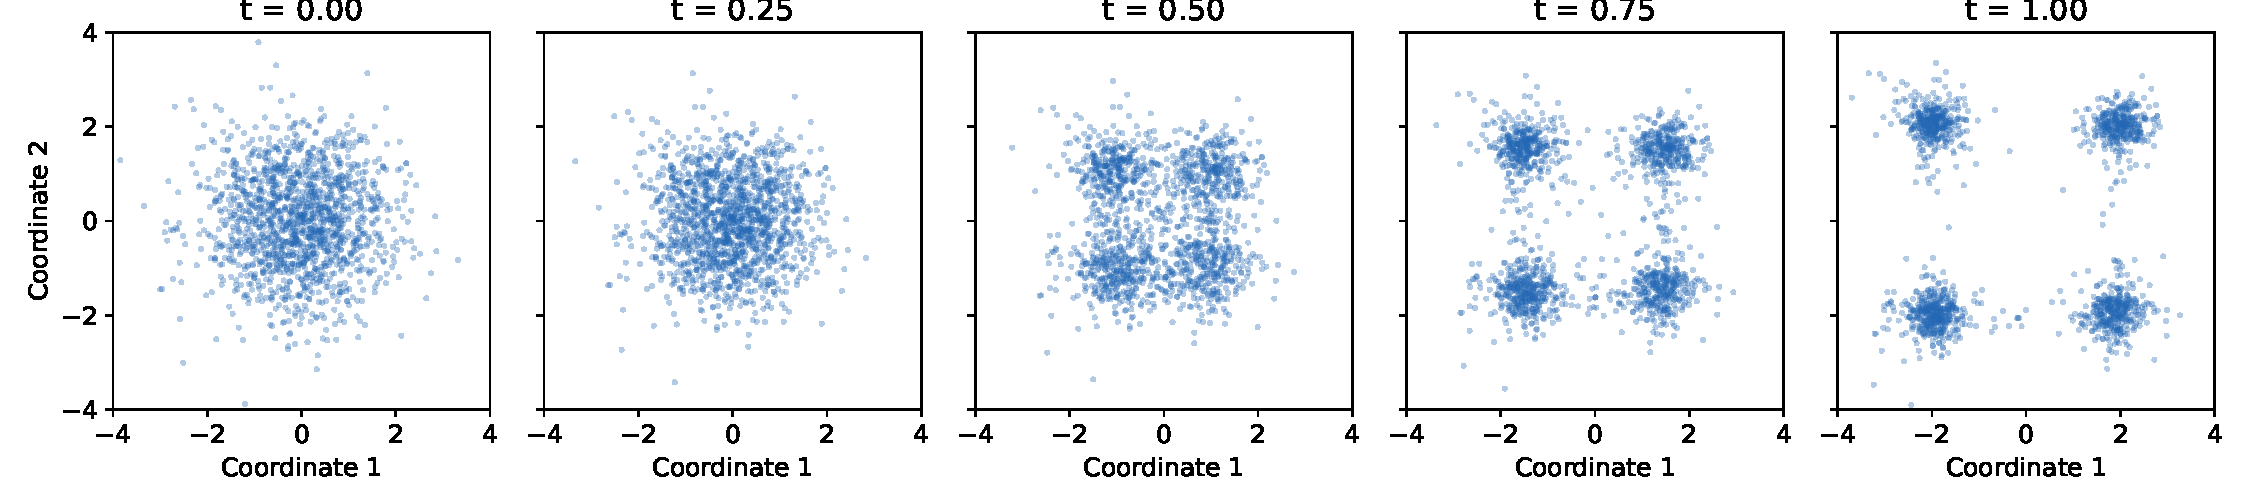
\includegraphics[width=\textwidth]{figures/generation_stages.pdf}
\end{center}
\vspace{5mm}
The panels follow the same 1,500 generated particles.\\[3mm]
No new noise enters between Euler steps. Randomness comes from the starting points.
\end{frame}

\begin{frame}{Individual generated trajectories}
\begin{columns}[c]
\begin{column}{.58\textwidth}
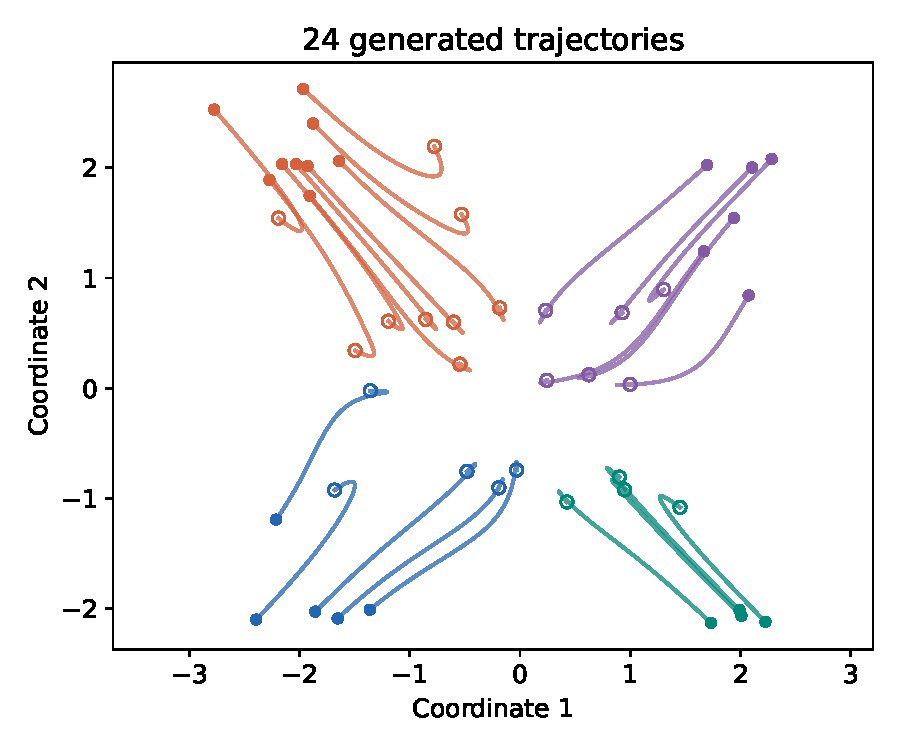
\includegraphics[width=\linewidth,height=.70\textheight,keepaspectratio]{figures/trajectories.pdf}
\end{column}
\begin{column}{.38\textwidth}
\small
24 trajectories from the learned ODE.\\[4mm]
Open circles: Gaussian starts.\\[4mm]
Filled dots: generated endpoints.\\[4mm]
Colors identify the nearest final center.\\[4mm]
These paths can curve, although the training interpolations were straight.
\end{column}
\end{columns}
\end{frame}

\begin{frame}{7. Fresh real and generated samples}
\begin{center}
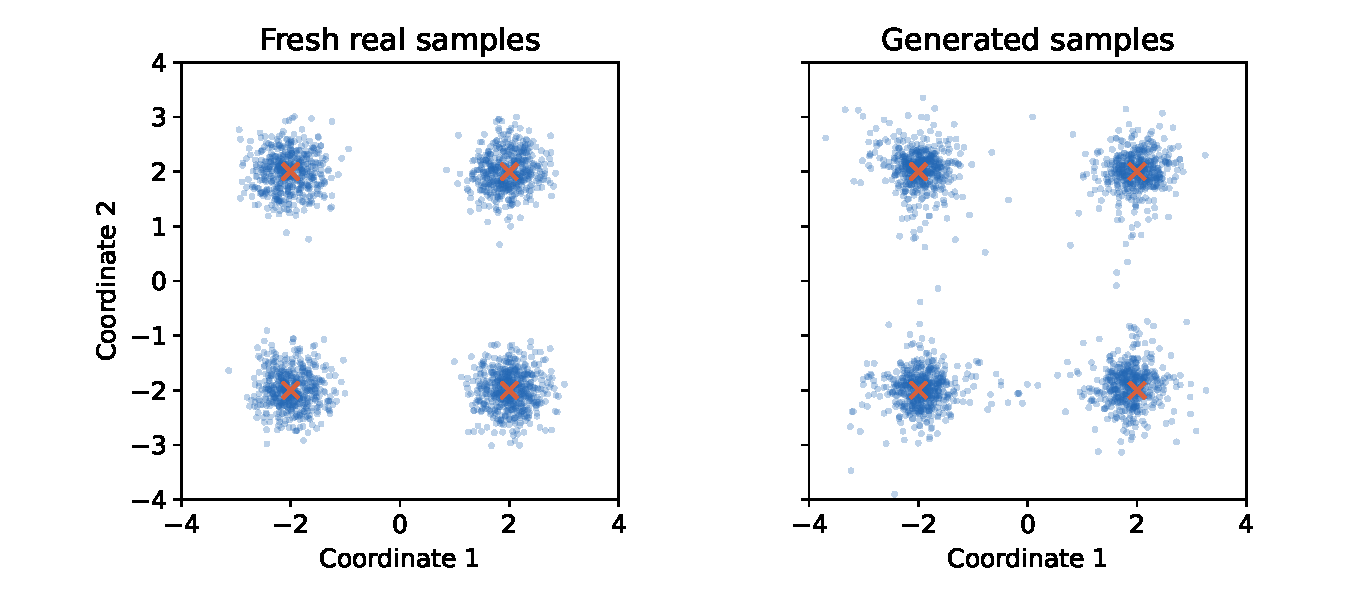
\includegraphics[width=.94\textwidth,height=.66\textheight,keepaspectratio]{figures/sample_comparison.pdf}
\end{center}
\small
Both panels use equal coordinate scales and display 2,000 points.\\[2mm]
We compare distributions, not a generated point with a paired correct endpoint.
\end{frame}

\begin{frame}[fragile]{Checking all four clusters and their spread}
\begin{lstlisting}[basicstyle=\ttfamily\footnotesize]
distance, group = torch.cdist(points, centers).min(dim=1)
shares = 100 * torch.bincount(group, minlength=4) / len(points)
radius = distance.square().mean().sqrt()
nearby = 100 * (distance < 1).float().mean()
\end{lstlisting}
\vspace{3mm}
\begin{itemize}\setlength\itemsep{3mm}
\item Mode shares: does each center receive roughly 25\% of samples?
\item RMS distance: how spread out are samples around their nearest centers?
\item Within radius 1: how much mass lies near the clusters?
\end{itemize}
\small Nearest-center assignments are diagnostics, not inferred true component labels.
\end{frame}

\begin{frame}{Results on 5,000 new samples}
\begin{center}
\small\begin{tabular}{lrr}
\toprule
Diagnostic & Fresh real & Generated\\
\midrule
Nearest $(-2,-2)$ (\%) & 24.9000 & 25.9800\\[1mm]
Nearest $(-2,2)$ (\%) & 24.3800 & 25.8400\\[1mm]
Nearest $(2,-2)$ (\%) & 25.8600 & 23.9600\\[1mm]
Nearest $(2,2)$ (\%) & 24.8600 & 24.2200\\[1mm]
RMS distance to nearest center & 0.4934 & 0.5187\\[1mm]
Within distance 1 of a center (\%) & 98.4400 & 95.2000\\[1mm]
\bottomrule
\end{tabular}

\end{center}
\vspace{3mm}
Finite-sample proportions differ from the theoretical 25\% per component.\\[3mm]
Good mode counts alone are insufficient. Four collapsed points could have the same counts.
\end{frame}

\begin{frame}{An experiment: 1, 10, or 100 Euler steps}
\begin{center}
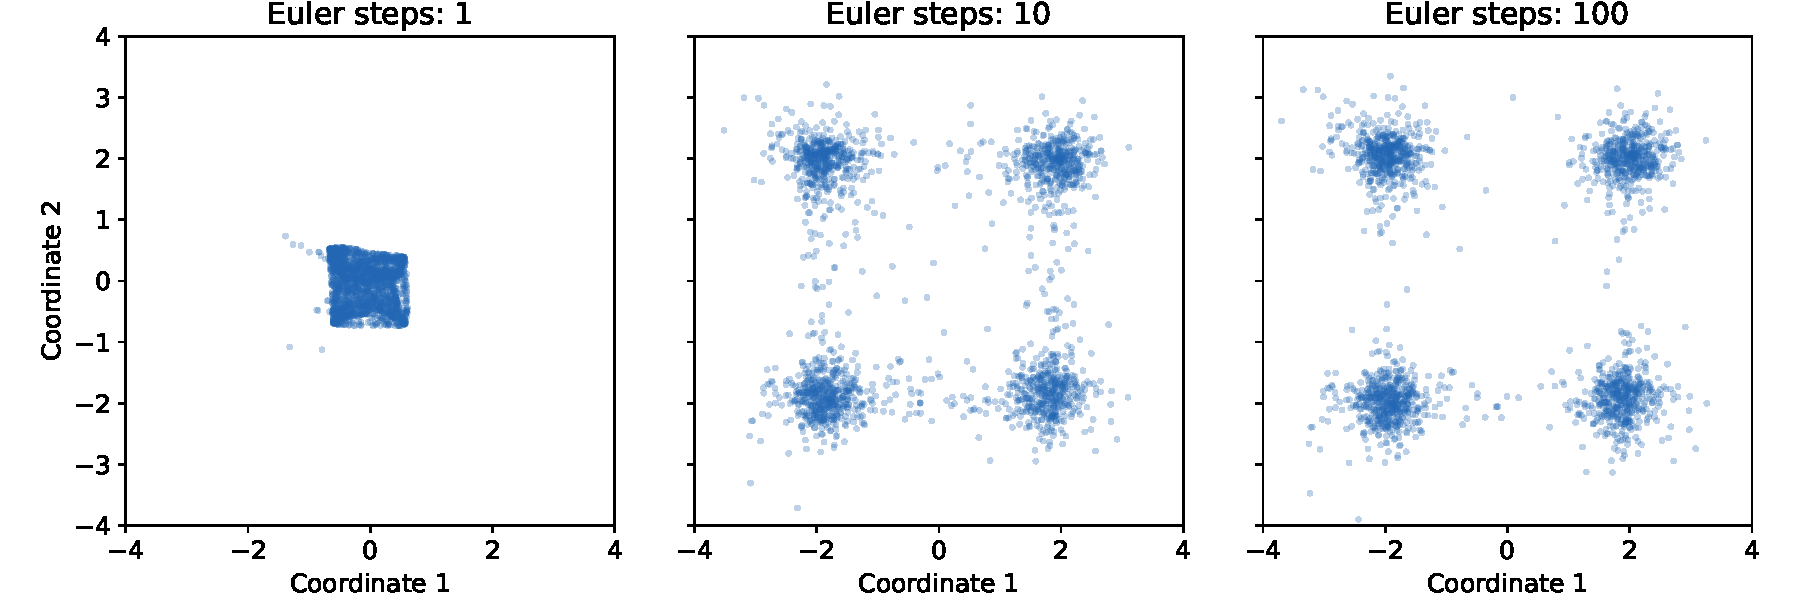
\includegraphics[width=\textwidth,height=.65\textheight,keepaspectratio]{figures/euler_steps.pdf}
\end{center}
\small
Same model and same initial noise in all three panels. No retraining.\\[2mm]
For the zero-mean target, $v^*(x,0)=-x$: one unit Euler step gives $x-x=0$.\\[2mm]
Smaller steps reduce numerical error; they cannot repair a poorly learned field.
\end{frame}

\begin{frame}{Diffusion models also have an ODE sampler}
\small For a forward diffusion with scalar, state-independent noise coefficient:
\normalsize
\[dX=f(X,\tau)\,d\tau+g(\tau)\,dW_\tau\]
\[\frac{dX}{d\tau}=f(X,\tau)-\frac12g(\tau)^2\nabla_x\log p_\tau(X)\]
\small
$W_\tau$ supplies Brownian noise; $\nabla_x\log p_\tau$ is the score.\\[3mm]
With the exact score and regularity assumptions, the SDE and probability-flow ODE have the same one-time distributions, not the same paths.\\[3mm]
Diffusion generation runs this ODE backward from noise to data. Our notebook directly learns a velocity with $t$ increasing from noise to data.
\vfill{\tiny\color{gray}Song et al., \href{https://arxiv.org/abs/2011.13456}{Score-Based Generative Modeling through Stochastic Differential Equations}, Section 4.3.}
\end{frame}

\begin{frame}{What the example establishes}
\begin{itemize}\setlength\itemsep{4mm}
\item A velocity network and an ODE solver can turn Gaussian inputs into a multimodal sample distribution.
\item Finite data, approximation, optimization, and the solver all contribute error.
\item Generation time is an artificial parameter. These two-dimensional outputs are not time series.
\item A future model could generate an entire time series and evaluate temporal structure using suitable tools, potentially including Volterra signatures.
\end{itemize}
\end{frame}

\begin{frame}{Experiments and further reading}
\begin{enumerate}\setlength\itemsep{3mm}
\item Change the seed and compare cluster coverage and spread.
\item Train for 1,000 iterations, keeping 100 sampling steps.
\item Make the target clusters narrower by reducing \texttt{sigma}.
\item Remove the time input from both training and sampling. What changes?
\end{enumerate}
\vspace{3mm}
Restart the kernel for each experiment. Use fresh test samples after tuning.
\vfill
\tiny References: \href{https://arxiv.org/abs/2210.02747}{Lipman et al., Flow Matching};
\href{https://arxiv.org/abs/2209.03003}{Liu et al., Rectified Flow};
\href{https://arxiv.org/abs/2011.13456}{Song et al., Score-Based Generative Modeling}.\\[3mm]
\small Companion notebook: \texttt{learning\_flow\_matching.ipynb}
\end{frame}

\end{document}
